\documentclass[10pt,onecolumn]{book}

\usepackage{times} % font
\usepackage{graphicx} % picture reference
\usepackage{amsmath} % split of mathematical formulas
\usepackage{amssymb} % special mathematical symbols
\usepackage{geometry} % margin
\usepackage{setspace} % letter-spacing
\usepackage{indentfirst} % indent
\geometry{left=2cm,right=2cm, top=2cm, bottom=2cm}
\usepackage{hyperref} % hyperlink
\usepackage{cite}
\usepackage[sectionbib]{chapterbib}

\usepackage{multirow}
%\usepackage{color}
\usepackage{ulem}
%\usepackage{todonotes}
\usepackage{xargs}
\usepackage[pdftex,dvipsnames]{xcolor}
\usepackage[colorinlistoftodos,prependcaption]{todonotes}
\newcommandx{\note}[2][1=]{\todo[linecolor=yellow,backgroundcolor=yellow!25,bordercolor=yellow,#1]{#2}}
\newcommandx{\unsure}[2][1=]{\todo[linecolor=red,backgroundcolor=red!25,bordercolor=red,#1]{#2}}
\newcommandx{\improvement}[2][1=]{\todo[linecolor=Plum,backgroundcolor=Plum!25,bordercolor=Plum,#1]{#2}}

%\numberwithin{equation}{section} % the number of equation

%\usepackage{fancy}%页眉页脚包
%\pagestyle{plain}%页眉页脚设置
\usepackage{fancyhdr}
\pagestyle{fancy}

\usepackage{boxedminipage}
\usepackage{algorithm, algorithmic}


\def\ie{\emph{i.e.}}
\def\eg{\emph{e.g.}}
\def\etal{\em {et al.}}

\newcommand{\bm}[1]{\mbox{\boldmath{$#1$}}}
\newcommand{\figref}[1]{Fig. \ref{#1}}
\newcommand{\tabref}[1]{Tab. \ref{#1}}
\newcommand{\equref}[1]{(\ref{#1})}
\newcommand{\secref}[1]{Sect. \ref{#1}}
\newcommand{\algref}[1]{Alg. \ref{#1}}
\newcommand{\myPara}[1]{\vspace{.05in}\noindent\textbf{#1}}
\newcommand{\rev}[1]{\textcolor{blue}{#1}}
\newcommand{\rr}[1]{\textcolor{red}{#1}}
\newcommand{\cg}[1]{\textcolor{green}{#1}}
\newcommand{\bb}[1]{\textcolor{blue}{#1}}
\newcommand{\bl}[1]{\textbf{#1}}
\newcommand{\ul}[1]{\underline{#1}}
\newcommand{\mc}[1]{\mathcal{#1}}
\newcommand{\mb}[1]{\mathbb{#1}}

\begin{document}
\date{}

\title{\textbf{Mathematics, Machine Learning and Deep Learning Notes}}

\author{Jinming Su}
\date{Last update: \today}

\maketitle

\thispagestyle{empty}
\newpage
\pagenumbering{Roman}
\newpage
\tableofcontents
%\newpage
%\listoffigures
%\newpage
%\listoftables
%\newpage
%\pagenumbering{arabic}
\newpage
\listoftodos

\newpage
\pagenumbering{arabic}
\mainmatter

\chapter{Mathematical Foundation}
\section{Probability theory and mathematical statistics}
\textbf{Probability theory} mainly focuses on the probability of occurrence of a single event, while \textbf{mathematical statistics} is more inclined to statistics. It focuses on the sampling probability of a group and the possible interval of occurrence of this probability.

In the following introduction, these two concepts are introducted without distinction. 

\subsection{How to get expected value and variance?}
$X$ is a random variable whose values are $X_{1}, X_{2}, ..., X_{n}$. $P(X_{1}), P(X_{2}), ..., P(X_{n})$ are the probability corresponding to these values. The expected value of $X$ can be denoted as $E(X)$, and the variance is denoted as $Var(X)$. Then, 
\begin{equation}
\begin{split}
	E(X) & = \sum_{i = 1}^{n} X_{i}P(X_{i}) \text{\ for discrete variable} \\
		 & = \int_{X}xf(x)dx \text{\ for continous variable} \\	
\end{split},
\end{equation}
and
\begin{equation}
\begin{split}
	Var(X) & = \sum_{i = 1}^{n} (X_{i} - E(X))^2 P(X_{i}) \text{\ for discrete variable} \\
		 & = \int_{X}(x - E(X))^2 f(x) dx  \text{\ for continous variable} \\	
\end{split}.
\end{equation}
For discrete variable, 
\begin{equation}
\begin{split}
	Var(X) & = \sum_{i = 1}^{n} (X_{i} - E(X))^2 P(X_{i}) \\
		   & = E[(X - E(X))^2] \\
		   & = E[X^2 + E(X)^2 - 2XE(X)] \\
		   & = E(X^2) + E(X)^2 - 2E(X)E(X) \\
		   & = E(X^2) - E(X)^2
\end{split}.
\end{equation}

\subsection{Discrete probability distribution}
\textbf{Bernoulli distribution} is \uline{the discrete probability distribution of a random variable} which takes the value 1 with probability $p$ and the value 0 with probability $q=1-p$. We denote Bernoulli distribution as $B(1, p)$. Mathematically, if $X$ is a random variable with $B(1, p)$, then $P(X=1)=p, P(X=0)=q=1-p$. The probability mass function $f$ of this distribution over possible outcoems k, is 
\begin{equation}
f(k;p) = 
\left\{
	\begin{array}{lr}
	p         & \mathrm{if} \ k = 1,\\
	q = 1 - p & \mathrm{if} \ k = 0. \\
	\end{array}
\right.
\end{equation}
The expected value and invarance  of a Bernoulli variable $X$ are
\begin{equation}\label{eq:bernoulli_distribution_e_var}
\left\{
	\begin{array}{lr}
	E(X) = P(X = 1) \cdot 1 + P(X = 0) \cdot 0 = p, \\
	E(X^2) = P(X = 1) \cdot 1^2 + P(X = 0) \cdot 0^2 = P(X = 1) = p, \\ 
	Var(X) = E(X^2) - E(X)^2 = p - p^2 = p(1 - p) = pq.
	\end{array}
\right.
\end{equation}
\note[inline]{Note in Eq.~\ref{eq:bernoulli_distribution_e_var}, maybe $P(X = 1)$ is equivalent $P(X^2 = 1^2)$, which ensures the establishment of this equation.}

\textbf{Binomial distribution} with parameters $n$ and $p$ is \uline{the discrete probability distribution of the number of successes in a sequence of n independent experiments.} Each experiment is a Bernoulli trial. In general, if the ramdom variable $X$ follows the binomial distribution with parameters $n \in \mathbb{N}$ and $p \in [0, 1]$, we write $X \sim B(n, p)$. The probability of getting exactly $k$ successes in $n$ trails is given by the probability mass function:
\begin{equation}
f(k; n, p) = P(k; n, p) = P(X = k) = \binom{n}{k} p^k (1-p)^{n-k}.
\end{equation}
The expected value and invariance of a Binomial variable $X$ are
\begin{equation}\label{eq:binomial_distribution_e_var}
\left\{
	\begin{array}{lr}
	\begin{split}
	E(X)  & = E(X_{1} + X_{2} + \cdot \cdot \cdot X_{n}) \\
		  & = E(X_{1}) + E(X_{2}) + \cdot \cdot \cdot + E(X_{n}) \\
		  & = p + p + \cdot \cdot \cdot + p \\
		  & = np, \\
	\end{split} \\
	\begin{split}
	Var(X) & = Var(X_{1}) + Var(X_{1}) + \cdot \cdot \cdot + Var(X_{1}) \\
		   & = nVar(X_{1}) \\
		   & = np(1-p). \\
	\end{split} 
	\end{array}
\right.
\end{equation}
\note[inline]{There exists another solution directly through derivation of the probability mass function of Binomial distribution.}

\textbf{Poisson distribution} is \uline{a discrete probability distribution that expresses the probability of a given number $k$ of events occurring in a fixed interval of time or space} if these events occure with a known constant rate $\lambda$ and independently of the time since the last events. If $X$ is a Poisson variable with the average number of events $\lambda$, we write $X \sim Possion(\lambda)$. The probability mass function is
\begin{equation}
f(k; n, \lambda) = P(X = k) = \frac{e^{-\lambda} \lambda^k}{k!}.
\end{equation}
The expected value and invariance of a Poission variable $X$ are
\begin{equation}\label{eq:poisson_distribution_e_var}
\left\{
	\begin{array}{lr}
	\begin{split}
	E(X)  & = \sum_{i=0}^{\infty} i P(X = i) \\
		  & = \sum_{i=1}^{\infty} i \frac{e^{-\lambda} \lambda^i}{i!} 
		    = \lambda e^{-\lambda} \sum_{i=1}^{\infty} \frac{\lambda^{i - 1}}{(i - 1)!} 
		    = \lambda e^{-\lambda} \sum_{i=0}^{\infty} \frac{\lambda^{i}}{i!} \\
		  & = \lambda e^{-\lambda} e ^ \lambda \\
		  & = \lambda \\
	\end{split} \\
	\begin{split}
	E(X^2) & = \lambda + \lambda ^ 2 \\
	\end{split} \\
	\begin{split}
	Var(X) & = \lambda + \lambda ^ 2 - \lambda^2 \\
		   & = \lambda \\
	\end{split}  \\
	\end{array}
\right.
\end{equation}
\note[inline]{Note there exists Taylor Expansion $e^x = 1 + \frac{x}{1!} + \frac{x^2}{2!} + \frac{x^3}{3!} + \cdot \cdot \cdot + \cdot \cdot \cdot = \sum_{i=0}^{\infty} \frac{x^i}{i!}$.} 
\improvement[inline]{Todo: Taylor's formula.}

\subsection{Continuous probability distribution}
For \textbf{continuous uniform distribution}, \uline{all intervals of the same length on the distribution's support are equally probable}. The support is defined by the two parameters, $a$ and $b$, which are its minimum and maximum values. The distribution is often abbreviated $U(a, b)$. The probability density function of the continuous uniform distribution is 
\begin{equation}
f(x)=
\left\{
	\begin{array}{ll}
		\frac{1}{b - a}  & \mathrm{for} \ a \le x \le b,  \\
		0                & \mathrm{for} \ x < a \ \mathrm{or} \ x > b. \\
	\end{array}
\right.
\end{equation}
The expected value and invariance of a Uniform variable $X$ are
\begin{equation}
\left\{
	\begin{array}{lr}
	\begin{split}
	E(X)  & = \int_{a}^{b} x \frac{1}{b - a} \\
		  & = \frac{x^2}{2(b - a)}\bigg|_{a}^b = \frac{b^2 - a^2}{2(b - a)} = \frac{(b + a)(b - a)}{2(b - a)} \\
		  & = \frac{b + a}{2}
	\end{split} \\
	\begin{split}
	E(X^2) & = \int_{a}^{b} x^2 \frac{1}{b - a} \\
		   & = \frac{x^3}{3(b - a)}\bigg|_{a}^b = \frac{b^3 - a^3}{3(b - a)} = \frac{(b - a)(b ^ 2 + a ^ 2 + ab)}{3(b - a)} \\
		   & = \frac{a ^ 2 + b ^ 2 + ab}{3} \\
	\end{split} \\
	\begin{split}
	Var(X) & = E(X^2) - E(X)^2 
		     = \frac{a ^ 2 + b ^ 2 + ab}{3} - (\frac{b + a}{2})^2 \\
		   & = \frac{4a ^ 2 + 4b ^ 2 + 4ab}{12} - \frac{3a^2 + 3b^2 + 6ab}{12} \\
		   & = \frac{(a - b)^2}{12}
	\end{split}  \\
	\end{array}
\right.
\end{equation}

The probability density function of the \textbf{normal distribution} is
\begin{equation}
f(x; \mu, \sigma^2) = \frac{1}{\sqrt{2 \pi \sigma^2}} e^{-\frac{(x - \mu)^2}{2\sigma^2}},
\end{equation}
where $\mu$ is the expectation and $\sigma$ is the standard deviation. If a random variable $X$ is distributed normally with mean $\mu$ and variance $\sigma^2$, one may write $X \sim N(\mu, \sigma^2)$. \note[inline]{The derivation of the expectation and invariance of normal distribution requires multiple integration operations.}

\textbf{Exponential distribution} is the probability distribution that describes the time between events in a Poisson point process, $i.e.$ a process in which event occur continuously and independently at a constant average rate. The distribution is often abbreviated $Exponential(\lambda)$. The probability density function of an exponential distribution is 
\begin{equation}
f(x;\lambda)=
\left\{
	\begin{array}{ll}
		\lambda e ^ {- \lambda x} \ & x \ge 0, \\
		0						    & x < 0.
	\end{array}
\right.
\end{equation}
The expected value and invariance of a Exponential variable $X$ are
\begin{equation}
\left\{
	\begin{array}{lr}
	E(X) = \frac{1}{\lambda}, \\
	Var(X) = \frac{1}{\lambda ^ 2}. \\	
	\end{array}
\right.
\end{equation}
\note[inline]{The derivation of the expectation and invariance of exponential distribution requires multiple integration operations.}
\improvement[inline]{Todo: Beta distribution.}

\subsection{Sample mean and sample variance}
\textbf{Sample mean} is defined as
\begin{equation}
\bar{X} = \frac{1}{n} \sum_{i=1}^n X_i.
\end{equation}

\textbf{Sample Variance} is defined as 
\begin{equation}
S^2 = \frac{1}{n - 1} \sum_{i=1}^n(X_i - \bar{X})^2.
\end{equation}

The above definitions follow the theorem: \uline{sample mean is unbiased estimation of population mean and sample variance is unbiased estimation of population variance.} 

\textbf{proof:}
\begin{equation}\label{eq:unbiased_estimation_of_sample_mean_and_variance}
\begin{split}
E[\bar{X}] &= E[\frac{1}{n} \sum_{i=1}^n X_i] \\
			&= \frac{1}{n} \sum_{i=1}^n E[X_i] \\
			&= \frac{1}{n} n E(X) \\
			&= E(X) \\
E[S^2] &= E[\frac{1}{n - 1} \sum_{i=1}^n(X_i - \bar{X})^2] \\
		&= \frac{1}{n-1}E[\sum_{i=1}^n(X_i ^ 2 + \bar{X} ^ 2 - 2 X_i \bar{X})] \\
		&= \frac{1}{n-1}(E[\sum_{i=1}^nX_i ^ 2] + n\bar{X}^2 - 2n\bar{X}^2) \\
		&= \frac{1}{n-1}(nE[X ^ 2] - nE[\bar{X}^2]) \\
		&= \frac{n}{n-1}(Var[X] + E[X]^2 - Var[\bar{X}] - E[\bar{X}]^2) \\
		&= \frac{n}{n-1}(Var[X] - Var[\bar{X}]) \\
		&= \frac{n}{n-1}(Var[X] - \frac{1}{n}Var[X]) \\
		&= Var[X]
\end{split}
\end{equation}

\section{Prior and posterior}
The prior probability is the probability of \uline{a cause inferred from experience}, denoted as $P(\theta)$. The posterior probability is the probability of \uline{the cause estimated from the result}, denoted as $P(\theta|x)$. The posterior probability is defined as 
\begin{equation}\label{eq:posterior}
\begin{split}
P(\theta|x) = \frac{P(x|\theta) P(\theta)}{P(x)}
\end{split}
\end{equation}
where $P(x|\theta)$ represents likelihood of $x$. \uline{In fact, likelihood is the function of parameters. Likelihood is equal to the probability of the result occurring caused by a cause (paramters) based on the cause. Likelihood is the viewpoint of the frequency. In the frequency, the parameter is a true value, not a random variable, so the parameter has no distribution and no probability.}

\chapter{Machine Learning}

\section{Why can't perceptron solve XOR problem?}
\begin{figure}[h]
\centering
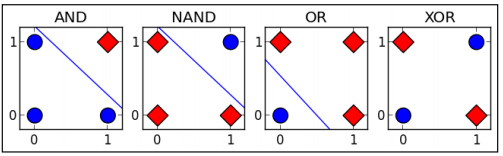
\includegraphics[width=0.4\textwidth]{figures/XOR_problem.png}
\caption{XOR problem.}
\end{figure}
 \uline{Linear classification models can't classify linear non-separable problems.} Perceptron is a linear classificatioin model, and XOR problem is a linear non-separable problem, so perceptron can't solve the XOR problem.

\subsection{Definition of perceptron}
Suppose the input space is $\mathcal{X} \subseteq \mathbb{R}^n$, and the output space is $\mathcal{Y} = \left\{+1, -1\right\}$. For an example $x \in \mathcal{X}$ where $x$ is an n-dimensional vector $(x_{1}, x_{2}, \cdot \cdot \cdot, x_{n})^\mathrm{T}$, $y \in \mathcal{Y}$ represents the category of $x$. Then, we get the perceptron model from the input space to output space: 
\begin{equation}
f(\vec{x}) = \mathrm{sign}(\vec{w}^\mathrm{T} \vec{x} + b),
\end{equation}
where $\vec{w}$ is weight and $b$ is bias. And $\mathrm{sign}$ is a sign function, $i. e.$
\begin{equation}
\mathrm{sign}(x)=
\left\{
	\begin{array}{ll}
		+1, \quad x \ge 0  \\
		-1, \quad x < 0
	\end{array}
\right.
\end{equation}

There exists \uline{a geometric interpretation} that a hyperpalne whose normal vector is $\vec{w}$ and intercept is $b$.

\subsection{Learning Algorithm}
Given a \uline{linear separable} dataset $T = {(x_{1}, y_{1}), (x_{2}, y_{2}), \cdot \cdot \cdot, (x_{N}, y_{N})}$, where $x_{i} \in \mathcal{X} \subseteq \mathbb{R}^n$, and $y_{i} \in \mathcal{Y} = {+1, -1}, i = 1, 2, \cdot \cdot \cdot, N$, we can construct a perspectron model to classify this dataset. 

(1) construct the loss function. we define the loss function as \uline{the total distance from misclassified points to hyperplane}. Toward this end, the distance from any point $x_{0}$ to hyperplane:
\begin{equation}
\frac{1}{||\vec{w}||} |\vec{w}^\mathrm{T}  \cdot \vec{x_{0}} + b|
\end{equation}
where ${||\vec{w}||}$ means the $L_{2}$ norm of $\vec{w}$.\\
\indent As for missclassified points, $\vec{w}^\mathrm{T}  \cdot \vec{x_{0}} + b > 0$ when $y_{i}=-1$, and $\vec{w}^\mathrm{T}  \cdot \vec{x_{0}} + b < 0$ when $y_{i}=+1$. So the total distance from all the misscalssified points to hyperplane is 
\begin{equation}\label{eq:perceptron_loss}
-\frac{1}{||w||}\sum_{\vec{x_{i}} \in M} y_{i} (\vec{w}^\mathrm{T}  \cdot \vec{x_{i}} + b),
\end{equation}
where $M$ is the set of misclassfied points.

\indent \uline{In Eq.~\ref{eq:perceptron_loss}, $\frac{1}{||w||}$ can be ignored. The reason is (a) $\frac{1}{||w||}$ doesn't affcet postive or negative judgment of $y_{i} (\vec{w}^\mathrm{T}  \cdot \vec{x_{i}} + b)$ and (b) $\frac{1}{||w||}$ doesn't affcet the final optimization result of Eq.~\ref{eq:perceptron_loss}. The final optimization result is there are no points with wrong classification, which leads to the loss of 0.} Toward this end, the loss function of preceptron is 
\begin{equation}\label{eq:perceptron_loss}
L(\vec{w}, b) = - \sum_{\vec{x_{i}} \in M} y_{i} (\vec{w}^\mathrm{T}  \cdot \vec{x_{i}} + b),
\end{equation}
and the optimization object is 
\begin{equation}\label{eq:perceptron_loss}
\min_{\vec{w}, b}L(\vec{w}, b) = \min_{\vec{w}, b}- \sum_{\vec{x_{i}} \in M} y_{i} (\vec{w}^\mathrm{T}  \cdot \vec{x_{i}} + b).
\end{equation}

(2) We adopt stochastic gradient descent algorithm to train the perceptron model. Suppose the set of misclassified points is fixed, thus the gradient of loss function $L(\vec{w}, b)$:
\begin{equation}
\begin{split}
	\nabla_{\vec{w}}L(\vec{w}, b) & = - \sum_{\vec{x_i} \in M} y_i \vec{x_i} \\
	\nabla_{b}L(\vec{w}, b)       & = - \sum_{\vec{x_i} \in M} y_i
\end{split}.
\end{equation}
So, the stratagies of $\vec{w}$ and $b$ based on one misclassified point are:
\begin{equation}\label{eq:perceptron_parameter_update}
\begin{split}
	\vec{w} & \gets \vec{w} + \eta y_i \vec{x} \\
	b & \gets b + \eta y_i
\end{split},
\end{equation}
where $\eta$ is the learning rate.

(3) The standard form of perceptron learing algorithm: \\
\indent	\indent input: \uline{linear seperable training set}: $T = \left\{ (x_1, y_1), (x_2, y_2), \cdots, (x_n ,y_n) \right\}$, where $\vec{x_i} \in \mathcal{X} \subseteq \mathbb{R}^n$ and $y_i \in \mathcal{Y} = \left\{-1, +1\right\}, i = 1, 2, \cdots, N$. In addition, the learning rate is denoted 
as $\eta (0 < \eta \le 1)$. \\
\indent \indent output: $\vec{w}, b$. And the perceptron model $f(\vec{x}) = \mathrm{sign}(\vec{w}^\mathrm{T} \vec{x} + b)$. \\
\indent \indent (a) choose initial values, $\vec{w_0}, b_0$, and usually $\vec{w_0} = 0, b_0 = 0$; \\
\indent \indent (b) choose one example $(\vec{x_i}, y_i)$ from the traning set; \\
\indent \indent (c) if $y_{i} (\vec{w}^\mathrm{T}  \cdot \vec{x_{i}} + b) \le 0$:
\begin{equation}
\begin{split}
\vec{w} & \gets \vec{w} + \eta y_i \vec{x} \\
	b & \gets b + \eta y_i
\end{split};
\end{equation} \\
\indent \indent (d)go to (b) until there are no misclassified points in training set.


(4) \note[inline]{The convergence of this algorithm about perceptron leraning can be proved, but it is not within the scope of this note at present.}

\subsection{Dual form of perceptron learning algorithm}
From Eq.~\ref{eq:perceptron_parameter_update}, $\vec{w}$ and $b$ are updated for many times. Suppose the number of updates about each example is $n_i (i = 1, 2, \dots N)$, and we define $\alpha_i = n_i \eta$. Then, the final learned $\vec{w}$ and $b$ can be expressed as
\begin{equation}
\begin{split}
	\vec{w} & = \sum_{i = 1}^{N} \alpha_i y_i \vec{x_i} \\
	b 		& = \sum_{i = 1}^{N} \alpha_i y_i
\end{split}.
\end{equation}

Then, we can obtain the dual form of perceptron learning algorithm.\\
\indent	\indent input: \uline{linear seperable training set}: $T = \left\{ (x_1, y_1), (x_2, y_2), \cdots, (x_n ,y_n) \right\}$, where $\vec{x_i} \in \mathcal{X} \subseteq \mathbb{R}^n$ and $y_i \in \mathcal{Y} = \left\{-1, +1\right\}, i = 1, 2, \cdots, N$. In addition, the learning rate is denoted 
as $\eta (0 < \eta \le 1)$. \\
\indent \indent output: $\vec{\alpha} = (\alpha_1, \alpha_2, \cdots, \alpha_N)^\mathrm{T}, b$. And the perceptron model $f(\vec{x}) = \mathrm{sign}(\sum_{j=1}^{N} \alpha_j y_j \vec{x_j}^\mathrm{T} \vec{x} + b )$. \\
\indent \indent (a) choose initial values, $\vec{\alpha}, b_0$, and usually $\vec{\alpha} = 0, b_0 = 0$; \\
\indent \indent (b) choose one example $(\vec{x_i}, y_i)$ from the traning set; \\
\indent \indent (c) if $y_{i} (\sum_{j=1}^{N} \alpha_j y_j \vec{x_j}^\mathrm{T} \vec{x} + b) \le 0$:
\begin{equation}
\begin{split}
\vec{\alpha_i} & \gets \alpha_i + \eta \\
	b & \gets b + \eta y_i
\end{split};
\end{equation} \\
\indent \indent (d)go to (b) until there are no misclassified points in training set.

\section{How to get the update rule of parameters of backpropagation in gradient descent algorithm?}
An intuitive and imprecise proof is as follows. Assuming that there is a differentiable loss function $\mathcal{L}$ on training set with respect to parameter $\vec{w} = (w_1, w_2, \cdots, w_n)$ of the training model. Then, the total increment of $\mathcal{L}$ is
\begin{equation}
\begin{split}
\Delta \mathcal{L} & = \frac{\partial \mathcal{L}}{\partial w_1} \Delta w_1 + \frac{\partial \mathcal{L}}{\partial w_2} \Delta w_2 + \cdots + \frac{\partial \mathcal{L}}{\partial w_n} \Delta w_n + o(\rho) \\
				   & \approx \frac{\partial \mathcal{L}}{\partial w_1} \Delta w_1 + \frac{\partial \mathcal{L}}{\partial w_2} \Delta w_2 + \cdots + \frac{\partial \mathcal{L}}{\partial w_n} \Delta w_n
\end{split}.
\end{equation}
Define $\nabla \mathcal{L}_{\vec{w}} = (\frac{\partial \mathcal{L}}{\partial w_1}, \frac{\partial \mathcal{L}}{\partial w_2}, \cdots, \frac{\partial \mathcal{L}}{\partial w_n})^\mathrm{T}$, which represents the vector of gradients. Therefore, 
\begin{equation}
\Delta \mathcal{L} \approx \nabla \mathcal{L}_{\vec{w}}^\mathrm{T} \cdot \Delta \vec{w}.
\end{equation}
Our goal is to reduce the loss function $\mathcal{L}$, which is equivalent to making the total increment $\Delta \mathcal{L}$ negative. Toward this end, construct 
\begin{equation}
\Delta \vec{w} = -\eta \nabla \mathcal{L}_{\vec{w}},
\end{equation}
which ensure that $\Delta \mathcal{L} \approx \nabla \mathcal{L}_{\vec{w}}^\mathrm{T} \cdot \Delta \vec{w} = - \eta ||\nabla \mathcal{L}_{\vec{w}}^\mathrm{T}||_2^2 \le 0$. So, the update rule of parameter $\vec{w}$ is 
\begin{equation}
\vec{w} \gets \vec{w} -\eta \nabla \mathcal{L}_{\vec{w}}.
\end{equation}
\uline{In other word, in gradient descent algorithm, the direction of parameter update is opposite to its gradient direction.}

\section{Generative model and discriminative model}
(1) Generative model: perceptron

\section{Support vector machine}
\improvement[inline]{Todo: SVM}

\improvement[inline]{Todo: Random forest}

\chapter{Deep Network}
\section{How does backpropagation work?}
\begin{figure}[h]
\centering
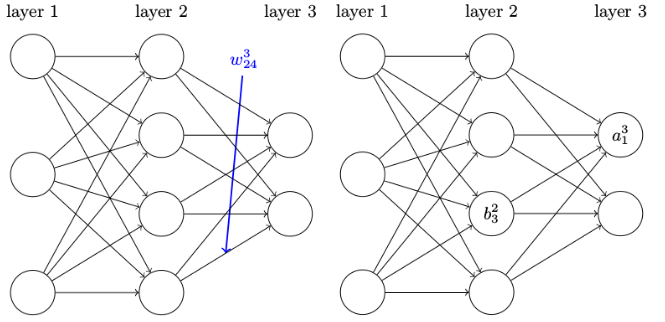
\includegraphics[width=0.5\textwidth]{figures/neural_network.png}
\caption{Neural network.}
\end{figure}
First, symbol definition is carried out. We use $w^l_{jk}$ to denote the weight for the connection from the $k$th neuron in the $(l - 1)$th layer to the $j$th neuron in the $l$th layer. Moreover, we use $b^l_j$ for the bias of $j$th neuron in $l$th layer and we use $a^l_j$ for the activation of the $j$th neuron in $l$th layer. We also use $z^l_j$ as the \uline{weighted input}  of $j$th neuron in $l$th layer. Then
\begin{equation}
\begin{split}
z^l_j & = \sum_k w^l_{jk} a^{l - 1} _ k + b^l_j, \\
a^l_j & = \sigma(\sum_k w^l_{jk} a^{l - 1} _ k + b^l_j) \\
	  & = \sigma(z^l_j).
\end{split}
\label{eq:neural_network}
\end{equation}
where $\sigma$ is the activation function, such as Sigmoid function. Then, Eq.~\ref{eq:neural_network} can be expresented in a vector form. In detail, we use $\vec{a^l}$ for the activation vector in $l$th layer. $\vec{z^l}$ is the same. Moreover, we use $\bm{w^l}$ for the \uline{weight matrix} and $\vec{b^l}$ for the bias vector in $l$th layer. Then, 
\begin{equation}
\begin{split}
\vec{z^l} & = \bm{w^l}a^{l - 1} + b^l, \\
\vec{a^l} & = \sigma(\bm{w^l}a^{l - 1} + b^l) \\
		  & = \sigma(\vec{z^l}).
\end{split}
\end{equation}

The understanding of backpropagation is about how to chang the weights and biases in a network to change the cost function. Utimately, this means computing the partial derivatives $\frac{\partial \mathcal{L}}{\partial w^l_{jk}} $ and $\frac{\partial \mathcal{L}}{\partial b^l_j} $. To compute those, we first introduce an intermedia quantity $\delta^l_j$, which we call the \uline{error} of the $j$th neuroon in the $l$th layer. In the actual calculation process, backpropagation will give us a predure to compute $\delta^l_j$, and then will relate $\delta^l_j$ to $\frac{\partial \mathcal{L}}{\partial w^l_{jk}} $ and $\frac{\partial \mathcal{L}}{\partial b^l_j} $.

We define the error of the $j$th neuroon in the $l$th layer by
\begin{equation}
\delta^l_j = \frac{\partial \mathcal{L}}{\partial z^l_j}.
\end{equation}
Then, we can get \uline{the error of the output layer} $\delta^L$, and the components of $\delta^L$ are given by
\begin{equation}\label{eq:backpropagation_1}
\begin{split}
\delta^L_j & = \frac{\partial \mathcal{L}}{\partial z^L_j} 
		   = \frac{\partial \mathcal{L}}{\partial a^L_j}\frac{\partial a^L_j}{\partial z^L_j} \\
		   & = \frac{\partial \mathcal{L}}{\partial a^L_j} \sigma'(z^L_j).
\end{split}
\tag{BP1}
\end{equation}
Moreover, we can give the matrix-based form of Eq.~\ref{eq:backpropagation_1} by
\begin{equation}
\overrightarrow{\delta^L} = \nabla_{\overrightarrow{a^L}} \otimes \sigma'(\overrightarrow{z^L}).
\end{equation}

Then, we can obtain \uline{the error $\delta^l$ in terms of the error in the next layer $\delta^{l+1}$}. In particular, 
\begin{equation}\label{eq:backpropagation_2}
\begin{split}
\delta^l_j & = \frac{\partial \mathcal{L}}{\partial z^l_j} 
		    = \sum_k \frac{\partial \mathcal{L}}{\partial z^{l+1}_k} \frac{\partial z^{l+1}_k}{\partial z^l_j}
		    = \sum_k \delta^{l+1}_k \frac{\partial z^{l+1}_k}{\partial z^l_j} \\
		   & = \sum_k \delta^{l+1}_k \frac{\partial \sum_j w^{l+1}_{kj} \sigma(z^l_j) + b^l_k}{\partial z^l_j} \\
		   & = \sum_k \delta^{l+1}_k w^{l+1}_{kj} \sigma'(z^l_j)
\end{split}
\tag{BP2}
\end{equation}
Moreover, we can give the matrix-based form of Eq.~\ref{eq:backpropagation_2} by
\begin{equation}
\begin{split}
\overrightarrow{\delta^l} = ((\overrightarrow{w^{l+1}})^\mathrm{T}\delta^{l+1}) \otimes \sigma'(\overrightarrow{z^l}).
\end{split}
\end{equation}

Next, we can obtain \uline{the rate of change of the cost with respect to any weight in the network}. In particlular, 
\begin{equation}\label{eq:backpropagation_3}
\begin{split}
\frac{\partial \mathcal{L}}{\partial w^l_{jk}} & = \frac{\partial \mathcal{L}}{\partial z^l_j} \frac{\partial z^l_j}{\partial w^l_{jk}}
	= \frac{\partial \mathcal{L}}{\partial z^l_j} \frac{\partial \sum_k w^l_{jk} a^{l-1}_k + b^l_j}{\partial w^l_{jk}} \\
	& = \frac{\partial \mathcal{L}}{\partial z^l_j} a^{l - 1}_k \\
	& = \delta^l_j a^{l - 1}_k.
\end{split}
\tag{BP3}
\end{equation}
Moreover, we can give the matrix-based form of Eq.~\ref{eq:backpropagation_3} by
\begin{equation}
\frac{\partial \mathcal{L}}{\partial \bm{w^l}} = \overrightarrow{\delta^l} (\overrightarrow{a^{l-1}})^\mathrm{T}.
\end{equation}

We can obtain \uline{the rate of change of the cost with respect to any bias in the network}. In particlular, 
\begin{equation}\label{eq:backpropagation_4}
\begin{split}
\frac{\partial \mathcal{L}}{\partial b^l_j} & = \frac{\partial \mathcal{L}}{\partial z^l_j} \frac{\partial z^l_j}{\partial b^l_j}
	= \frac{\partial \mathcal{L}}{\partial z^l_j} \frac{\partial \sum_k w^l_{jk} a^{l-1}_k + b^l_j}{\partial b^l_j} \\
	& = \frac{\partial \mathcal{L}}{\partial z^l_j} \\
	& = \delta^l_j.
\end{split}
\tag{BP4}
\end{equation}
Moreover, we can give the matrix-based form of Eq.~\ref{eq:backpropagation_4} by
\begin{equation}
\frac{\partial \mathcal{L}}{\partial \overrightarrow{b^l}} = \overrightarrow{\delta^l}.
\end{equation}

\section{Why does batch normalization work?}
\subsection{Dataset shift and covariate shift}
There exists a inherent hypothesis in supervised learning: \uline{The training data in source domain and testing data in target domain are independent and identically drawn from the same distribution}. 

Usually, the distrbutions of training data and testing data are not exactly the same, especiallt when the training data is insufficient. This phenomenon is named as ``\uline{dataset shift}''. 

In analysis of covariance (ANOVA), convate is any continuous variable that is usually not controlled during data collection. (referring to \url{https://support.minitab.com/en-us/minitab/18/help-and-how-to/modeling-statistics/anova/supporting-topics/anova-models/understanding-covariates/}). 

For the input variable $x$ (also named as explanatory variable or covariate in scene of batch normalizatio), $y$ is the corresponding label, which is regarded as response variable. If the conditional probabilities of training data and testing data are the same but the marinal probabilities are different, $i.e.$
\begin{equation}\label{eq:covariate_shift}
\begin{split}
P_{tr}(y|x) & = P_{te}(y|x) \\
P_{tr}(x) & \ne p_{te}(y)
\end{split},
\end{equation}
we call this phenomenon as ``\uline{covariate shift}''. Covariate shift is a special kind of dataset shift. 

Moreover, we can deduce the Eq.~\ref{eq:covariate_shift} as follows:
\begin{equation}
\begin{split}
P_{tr}(x, y) = P_{tr}(y|x)P_{tr}(x) \\
P_{te}(x, y) = P_{te}(y|x)P_{te}(x)
\end{split},
\end{equation}
and we know the joint probabilities of traning data and testing data are different, $i. e.$, 
\begin{equation}\label{eq:covariate_shift_2}
P_{tr}(x, y) \ne P_{te}(x, y).
\end{equation}.
From Eq.~\ref{eq:covariate_shift_2}, this scene violates the independence hypothesis of supervised learning, so the prediction is inaccurate.

\unsure[inline]{A more precise definition of \textbf{covariate} can't be found.}

\subsection{Internal covariate shift}
\uline{Internal covariate shift} is defined as the change in the distribution of network activations due to the change in network parameters during training. 


\begin{figure}[h]
\centering
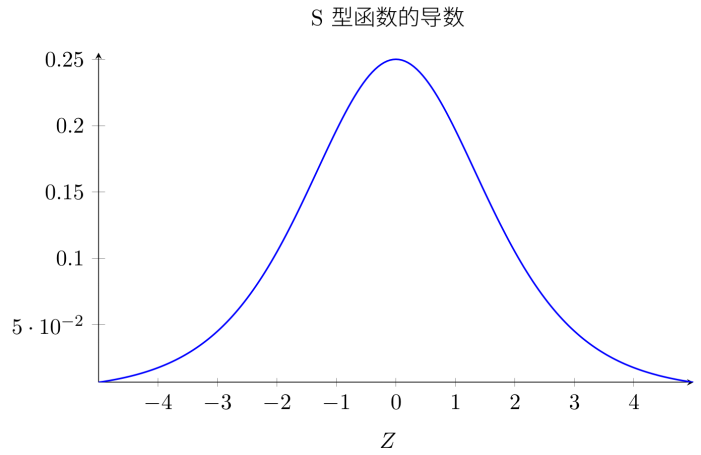
\includegraphics[width=0.5\textwidth]{figures/sigmoid.png}
\caption{Derivative of sigmoid function.}
\end{figure}


\textbf{Consequences of internal covariate shift: }(1) Intuitively, the layers need to continuously adapt to the new distribution, which lead to a decrease in training speed. (2) Objectively, the changes of $W$ and $b$ during training will likely move many dimensions of $x$ into the saturated regime of the nonlinearity ($e.g.$ sigmoid and tanh) and slow down the convergence. The saturation problem is usually addressed by using ReLU, careful initialization and small learning rates. Moreover, if the distribution of nonlinearity inputs remains more stable at the sensitive regions in nonlinearity as the network trains, the optimizer would be less likely to get stuck in the staturated regime, and the training would accelerate.

\improvement[inline]{PCA whitening and ZCA Whitening.}

\subsection{Batch normalization}
\textbf{Problem: } because whitening is expensive and maybe change the representation ability of a network by discarding the absolute scale of activations, batch nomalization emerges.

There are two treatments for batchnorm to address above two problems. (1) The first is instead of whitening the features in layer inputs and outputs jountly, batchnorm normalizes each scalar feature independently, by making it have the mean of 0 and the variance of 1. For a layer with $d$-dimensional input $x=[x^{(1)}, x^{(2)}, \cdots, x^{(k)}]$,  each dimension is normalized as follows 
\begin{equation}
\hat{x}^{(k)} = \frac{x^{(k)} - E[x^{(k)}]}{\sqrt{Var(x^{(k)})}}.
\end{equation}
(2)Simply normalizeing each input of a layer may reduce what the layer can represent. For example, nomalizing the inputs of a sigmoid would constrain them to the linear regime of the nonlinearity.
\begin{figure}[h]
\centering
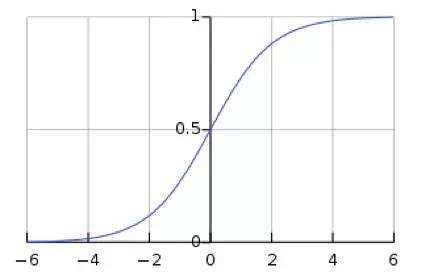
\includegraphics[width=0.5\textwidth]{figures/sigmoid_batchnorm.png}
\caption{Sigmoid function.}
\end{figure}
In this way, batchnorm turns the multi-layer nonlinear neural network into a multi-layer linear neural network, which is equivalent to the representation ability of a single layer linear network. The reduces the representation ability of the network. So, introduce $\gamma ^ {(k)}, \beta^{(k)}$ to scale and shift the normalized value:
\begin{equation}
y^{(k)} = \gamma ^ {(k)} \hat{x} ^ {(k)} + \beta ^ {(k)},
\end{equation}
which guarantee the representation ability of the network.
\improvement[inline]{Why is multi-layr linear network equivalent to the represetation ability of a single layer linear network.}

In addition, use mini-batch in stochatic gradient training, each mini-batch produces estimates of the man and variance of each activation. And obtain the forward algorithm of batch normalization as follows: \\

\begin{algorithm}
	\renewcommand{\algorithmicrequire}{\textbf{Input:}}
	\renewcommand{\algorithmicensure}{\textbf{Output:}}
	\caption{Forward algorithm of batch normalization.}
	\begin{algorithmic}[1]
		\REQUIRE values of $x$ over a mini-batch: $\mathcal{B}=\{x_1, x_2, \cdots, x_m\}$, parameters to be learned: $\gamma, \beta$
		\ENSURE$y_i = BN_{\gamma, \beta}(x_i)$
		\begin{equation}
		\begin{split}
		& \mu_\mathcal{B} \gets \frac{1}{m} \sum_{i=1}^m x_i \\
		& \sigma^2_\mathcal{B} \gets \frac{1}{m} \sum_{i=1}^m (x_i - \mu_\mathcal{B})^2 \\
		& \hat{x}_i \gets \frac{x_i - \mu_\mathcal{B}}{\sqrt{\sigma^2_\mathcal{B} + \epsilon}} \\
		& y_i \gets \gamma\hat{x}_i + \beta = BN_{\gamma, \beta}(x_i)
		\end{split}
		\notag
		\end{equation}
	\end{algorithmic}  
\end{algorithm}
In this manner, we know 
\begin{equation}
\begin{split}
E[\hat{x}] &= E[\frac{x_i - \mu_\mathcal{B}}{\sqrt{\sigma^2_\mathcal{B} + \epsilon}}] \\
		&= \frac{1}{\sqrt{\sigma^2_\mathcal{B} + \epsilon}} (E[x_i] - E[\mu_\mathcal{B}]) \\
		&= 0 \\
Var[\hat{x}] &= E[\hat{x}^2] - (E[\hat{x}])^2 \\
			&= E[(\frac{x_i - \mu_\mathcal{B}}{\sqrt{\sigma^2_\mathcal{B} + \epsilon}})^2] + 0 \\
			& = \frac{1}{\sigma^2_\mathcal{B} + \epsilon} E[(x_i - \mu_\mathcal{B})^2] \\
			& = \frac{1}{\sigma^2_\mathcal{B} + \epsilon} \sigma^2_\mathcal{B} \\
			& \approx 1
\end{split}.
\end{equation}
The distribution of values of any $\hat{x}$ has the expected value of 0 and the invariance of 1, as long as the elements of each mini-batch are sampled from the same distribution, and if we neglect $\epsilon$. This distribution can be seen as an approximate standard normal distribution $N(0, 1)$.

We compute the gradients with respect to the parameters of the BN thansform of loss $\mathcal{L}$ for backpropagation. The chain rule is used as follows:
\begin{equation}
\begin{split}
& \frac{\partial \mathcal{L}}{\partial \gamma} = \sum_i \frac{\partial \mathcal{L}}{\partial y_i}  \frac{\partial y_i}{\partial \gamma} = \sum_i \frac{\partial \mathcal{L}}{\partial y_i} \hat{x}_i, \\
& \frac{\partial \mathcal{L}}{\partial \beta} = \sum_i \frac{\partial \mathcal{L}}{\partial y_i}  \frac{\partial y_i}{\partial \beta} = \sum_i \frac{\partial \mathcal{L}}{\partial y_i}. \\
\end{split}
\end{equation}
\note[inline]{There exists $\sum_i$ for $y_i$ because gradient from each $y_i$ will backpropagate for $\gamma$ and the effect of summation is achieved.}
For the process of \textbf{backpropagation}, we also need to compute $\frac{\partial \mathcal{L}}{\partial x_i}$, which is got by:
\begin{equation}
\begin{split}
\frac{\partial \mathcal{L}}{\partial \hat{x}_i} & = \frac{\partial \mathcal{L}}{\partial y_i}  \frac{\partial y_i}{\partial \hat{x}_i} \\
&= \frac{\partial \mathcal{L}}{\partial y_i} \gamma 
\\
\frac{\partial \mathcal{L}}{\partial \sigma^2_\mathcal{B}} &= \sum_i \frac{\partial \mathcal{L}}{\partial \hat{x}_i}  \frac{\partial \hat{x}_i}{\partial \sigma^2_\mathcal{B}} \\
&= \sum_i \frac{\partial \mathcal{L}}{\partial \hat{x}_i} (x_i - \mu_\mathcal{B}) (-\frac{1}{2}) (\sigma^2_\mathcal{B} + \epsilon)^{-\frac{3}{2}} \\
&=-\frac{1}{2} \sum_i \frac{\partial \mathcal{L}}{\partial \hat{x}_i} (x_i - \mu_\mathcal{B}) (\sigma^2_\mathcal{B} + \epsilon)^{-\frac{3}{2}} 
\\
\frac{\partial \mathcal{L}}{\partial \mu_\mathcal{B}} &= \frac{\partial \mathcal{L}}{\partial \hat{x}_i} \frac{\partial \hat{x}_i}{\partial \mu_\mathcal{B}} + \frac{\partial \mathcal{L}}{\partial \sigma^2_\mathcal{B}} \frac{\partial \sigma^2_\mathcal{B}}{\partial \mu_\mathcal{B}} \\
&= \sum_i \frac{\partial \mathcal{L}}{\partial \hat{x}_i}(-1)(\sigma^2_\mathcal{B} + \epsilon)^{-\frac{1}{2}} + \frac{\partial \mathcal{L}}{\partial \sigma^2_\mathcal{B}}\frac{1}{m}\sum_i (-2) (x_i - \mu_\mathcal{B}) \\
&= -\sum_i \frac{\partial \mathcal{L}}{\partial \hat{x}_i}\frac{1}{\sqrt{\sigma^2_\mathcal{B} + \epsilon}} - \frac{\partial \mathcal{L}}{\partial \sigma^2_\mathcal{B}}\frac{2}{m}\sum_i(x_i - \mu_\mathcal{B})
\\
\frac{\partial \mathcal{L}}{\partial x_i} &= \frac{\partial \mathcal{L}}{\partial \hat{x}_i} \frac{\partial \hat{x}_i}{\partial x_i} + \frac{\partial \mathcal{L}}{\partial \sigma^2_\mathcal{B}} \frac{\partial \sigma^2_\mathcal{B}}{\partial x_i}+ \frac{\partial \mathcal{L}}{\partial \mu_\mathcal{B}} \frac{\partial \mu_\mathcal{B}}{\partial x_i} \\
&= \frac{\partial \mathcal{L}}{\partial \hat{x}_i} \frac{1}{\sqrt{\sigma^2_\mathcal{B} + \epsilon}} + \frac{2}{m} \frac{\partial \mathcal{L}}{\partial \sigma^2_\mathcal{B}} (x_i - \mu_\mathcal{B}) + \frac{1}{m} \frac{\partial \mathcal{L}}{\partial \mu_\mathcal{B}}
\\
\end{split}
\end{equation}

For the \textbf{inference} of the network, sometimes we want the output to depend only on the few or one input. At this time, $\mu$ and $\sigma^2$ are computed by each mini-batch $\mu_\mathcal{B}$ and $\sigma^2_\mathcal{B}$ by their unbiased estimations as proved in~\ref{eq:unbiased_estimation_of_sample_mean_and_variance}:
\begin{equation}
\begin{split}
\mu &= E(\mu_\mathcal{B}), \\
\sigma^2 &= \frac{n}{n-1}E(\sigma^2_\mathcal{B}), \\
BN(X) & = \gamma \frac{X - \mu}{\sqrt{\sigma^2 + \epsilon}} + \beta.
\end{split}
\end{equation}

The advantages of batch normalization is as follows: (1) batch normalization ensure the stable distributions of input in each layer, which reduces the learning pressure at the later layer and improves the learning speed; (2) batch normalization makes the model less sensitive to the parameters in the network, which simplifies the parameter adjustment precess, and makes the learning of this network more stable; (3) batch normalization can make the input of activation fall into the unsaturated region through the normalization operation, thus alleviating the problem of gradient vanishing.

\section{Why does residual learning work?}

\begin{figure}[h]
\centering
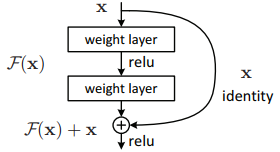
\includegraphics[width=0.4\textwidth]{figures/residual_learning_block.png}
\caption{Residual Learning.}
\end{figure}

In the process of optimization in deep networ
k, the input and output are usually close in the latter layers. In some latter layers, we define the input is $\rm{x}$ and the output is $\mathcal{H(\rm{x})}$. From above experience, we assume $\rm{x}$ and $\mathcal{H(\rm{x})}$ are close. Thus, the function of these layers is mapping from $\rm{x}$ to $\mathcal{H(\rm{x})}$. But usually this process is difficult becuase the relative gap between $\rm{x}$ and $\mathcal{H(\rm{x})}$ is small. Toward this end, we construct the residual as \uline{$\mathcal{F(\rm{x})} = \mathcal{H(\rm{x})} - \rm{x}$} to learning the gap. We can hypothesize that it is easier to optimize the residual mapping than to optimize the original mapping. To the extreme, if the mapping from input to output is indentity, it would be easier to push the residual to zero than to directly fit an identity mapping.

\uline{The real purpose of residual learning is that even if the network deepens, the performance of this network will not degenerate, thus ensuring the leaning of deeper network (even 1000 layers).}

\chapter{Contents specifically referenced}
\noindent $\bullet$ the chapter of (2)Perceptron in \cite{hangli2012}; \\
$\bullet$ BatchNorm from~\cite{ioffe2015batch};

{\small
\bibliographystyle{plain}
\bibliography{RefNote}
}

\end{document}
